\subsection{Descripción del problema.}

\vspace*{0.3cm}

Tenemos en cierta zona, pozos de petróleo que necesita ser refinado. Para que un pozo pueda refinar su petróleo, necesita o bien una refinería ubicada junto a él, o bien conectarse mediante tuberías a otro pozo que o tenga una refinería, o esté conectado mediante tuberías a algun pozo que puede refinar su petróleo. Nuestro objetivo es armar un plan de construcción que decida dónde construir una refinería y dónde construir un sistema de tuberías, de manera tal que todos los pozos puedan refinar su petróleo, minimizando el costo. Para esto, se tienen los siguientes datos:

\begin{itemize}
	\item Se conoce la cantidad de pozos en cuestión.
	\item Se conoce el costo de construir una refinería (este costo es fijo, y no varía según el pozo).
	\item Dada la geografía del lugar, no todo par de pozos se puede comunicar por una tubería directamente, y por decisiones de administración, una tubería no puede bifurcarse a mitad de camino entre un pozo y otro. Igualmente, conocemos todos los pares de pozos que pueden conectarse con una tubería, y el costo de ésta en caso de decidir construirse (a diferencia de las refinerías, las tuberías dependen del par de pozos que se quiere conectar).
	\item La complejidad del algoritmo debe ser estrictamente menor a $\mathcal{O}(n^3)$.
	\item La salida de este algoritmo debe contener una línea con el costo total de la solución, la cantidad de refinerías y la cantidad de tuberías a construir, seguido de una línea con los números de pozos en los que se construirán refinerías, más una línea con dos números por cada tubería a construir, representando el par de pozos conectados.	
\end{itemize}

Ejemplo:

Supongamos una zona petrolera como muestra la Figura \ref{fig:ejpetroleo}, donde los números de las aristas representan el costo de construir dicha tubería. Consideremos que el costo de construir una refinería es 75.

La solución para este ejemplo requiere construir 3 refinerías y 7 tuberías, cuyo costo total es 403. La Figura \ref{fig:ejpetroleores} muestra gráficamente la salida correcta.

\begin{figure}[!htb]
\minipage{0.5\textwidth}
\begin{center}
  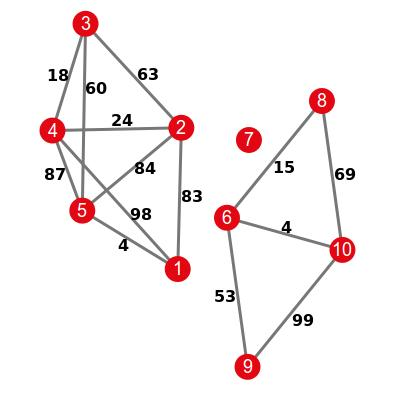
\includegraphics[scale=0.5]{imagenes/ejemplopetroleo.jpeg}
\end{center}
  \caption{Ejemplo de pozos y posibles tuberías}\label{fig:ejpetroleo}
\endminipage
\minipage{0.5\textwidth}
\begin{center}
  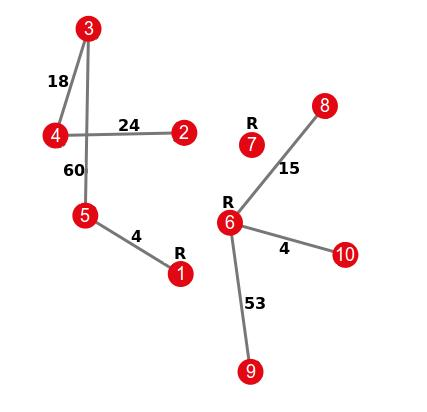
\includegraphics[scale=0.5]{imagenes/ejemplopetroleores.jpeg}
\end{center}
  \caption{Solución para el problema de la Figura \ref{fig:ejpetroleo}}\label{fig:ejpetroleores}
\endminipage
\end{figure}


\vspace*{0.6cm}

%\newpage
\subsection{Desarrollo de la idea y correctitud.}

\vspace*{0.3cm}

En primer lugar, notemos que el problema a resolver puede ser interpretado con grafos, considerando los pozos petroleros como nodos, y las posibles tuberías y sus costos como aristas con peso.  Tomando el problema de esta manera, podemos replantear el ejercicio como la búsqueda de un subgrafo que contenga a todos los nodos y escoja las aristas que minimicen el gasto.

Asumamos por un momento que todas las potenciales tuberías tienen un costo menor que construir una refinería, y que el grafo formado por los pozos y las tuberías posibles fuera conexo.  En este caso, el problema se puede traducir como la búsqueda de un árbol generador mínimo (AGM), ya que se trata de un subgrafo que recorre todos los nodos minimizando la suma de los pesos de las aristas.  Teniendo esta conexión entre los pozos, bastaría con tomar uno de ellos y colocar allí una refinería. Notemos que esto es correcto, ya que si tenemos todos los nodos conectados, con una sóla refinería es suficiente para que todos ellos refinen su petróleo, colocar más de una sólo incrementaría el costo y no mejoraría la situación.

Sin embargo, sabemos que no todo par de pozos puede conectarse mediante una tubería, y esto puede dar lugar a un grafo inicial no conexo.  De todos modos, si seguimos considerando que las tuberías son menos costosas que una refinería, bastaría con encontrar un AGM para cada componente conexa del grafo inicial, y colocar una refinería en cada uno de ellos. Esto minimizaría el gasto en cada componente y, por lo tanto, en toda la zona petrolera. 

Ahora bien, nada garantiza que toda potencial tubería tenga menor costo que una refinería. Supongamos que existe una solución al problema, es decir, existe un plan que permite refinar el petróleo de todos los pozos al menor costo, y supongamos que este plan tiene al menos una tubería con costo mayor al de una refinería. Siendo $r$ el costo de una refinería, $t > r$ el costo de alguna tubería de la solución mencionada, y A y B los nodos en los que incide dicha tubería, pueden darse los siguientes casos:

\begin{enumerate}
	\item Ambos pozos poseen una refinería. En este caso, si quitamos la tubería de costo $t$, A y B siguen pudiendo refinar su petróleo, al igual que todos los pozos conectados a ellos mediante tuberías. Es decir, la estructura resultante permite que todos los nodos refinen su petróleo y como quitamos una tubería, el costo del plan será menor.  Esto es absurdo, pues partimos del hecho de que la solución inicial era óptima.
	\item Sólo uno de los pozos tiene una refinería (digamos, A). Entonces tanto A como los nodos conectados a él pueden refinar su petróleo sin problemas. Si quitamos la tubería de costo $t$ puede suceder que:
	
	\begin{enumerate}
		\item B sigue pudiendo refinar su petróleo en otro lugar.  Entonces, al quitar la tubería de costo $t$ obtuvimos una nueva solución, y como quitamos una tubería, el costo del plan será menor.  Esto es absurdo, pues partimos del hecho de que la solución inicial era óptima.
		\item B refinaba su petróleo sólo a través de A y ahora ya no puede hacerlo. Si agregamos una refinería en el pozo B, volveríamos a refinar el petróleo de B y el de todos los nodos que se conectan con él. Y como $t > r$, el costo del nuevo plan sería menor, lo cual es absurdo, pues partimos del hecho de que la solución inicial era óptima.
	\end{enumerate}
	
	\item Ninguno de los dos pozos tienen refinería. Esto quiere decir que, mediante tuberías, A y B conectan a pozos que sí tienen refinería. Notemos que, si quitamos la tubería de costo $t$, no es posible que ambos dejen de poder refinar petróleo, pues eso significaría que aún con dicha tubería no podían hacerlo, y eso es absurdo.
	
	\begin{enumerate}
		\item Si quitamos la tubería de costo $t$ y ambos pozos siguen conectados a otros nodos con refinería, entonces ambos siguen refinando su petróleo junto con todos los nodos que llegan hasta ellos, y como quitamos una tubería, el costo del plan será menor.  Esto es absurdo, pues partimos del hecho de que la solución inicial era óptima.
		\item Si al quitar la tubería de costo $t$ alguno de los pozos, digamos A, deja de poder refinar su petróleo, podemos colocar una refinería allí y entonces tanto A como los pozos conectados a él vuelven a refinar su petróleo. Y como $t > r$, el costo del nuevo plan sería menor, lo cual es absurdo, pues partimos del hecho de que la solución inicial era óptima.
	\end{enumerate}
	
\end{enumerate}

[ACÁ YA NO SÉ CÓMO ACOMODAR POR LO DEL CASO T = R, FIJATE VOS ALE PLIS]
Los casos 1 y 3-a caen en absurdos para todo $t$ (en particular para $t > r$), así que ninguna solución podría tener esas características, y los casos 2 y 3-b caen en absurdos sólo para $t > r$. De esto se deduce que una solución óptima no tomará tuberías más caras que una refinería. Luego, como las tuberías que tengan un costo mayor a la construcción de una refinería no serán tomadas en cuenta, nos encontramos en el caso de que todas las tuberías a considerar tienen un costo menor a una refinería, y como dijimos anteriormente, puede resolverse mediante la búsqueda de AGM.  Como el caso $t = r$ no trae inconvenientes, las tuberías con ese costo serán igualmente consideradas.

Para buscar el AGM, nos hemos basado en el algoritmo de {\it Kruskal}.  Dado que este algoritmo opera sobre grafos conexos, lo hemos adaptado para poder procesar grafos que no necesariamente son conexos. Buscaremos que la solución hallada sea un bosque en el cual cada árbol sea un AGM de cada componente conexa inicial.

Para esto, primero acomodaremos todas las posibles tuberías ordenándolas crecientemente por costo. Así, de manera golosa, iremos tomándolas y colocándolas en la solución, garantizándonos un costo mínimo. A su vez, para asegurarnos de que el resultado sea un bosque, utilizaremos una tubería sólo si no forma circuitos con las colocadas anteriormente. Dado que al ir colocando aristas se van conectando distintos grupos de nodos, vamos a pensarlos como conjuntos disjuntos, de manera de poder consultar si dos nodos forman parte de un mismo conjunto o no.  Entonces, al tomar una arista podemos encontrarnos con los siguientes casos:

\begin{enumerate}
	\item La arista conecta dos nodos que no forman parte de ningún conjunto.  En este caso, asociaremos a ambos como parte de un nuevo conjunto.
	\item La arista conecta un nodo perteneciente a un conjunto con un nodo que no petenece a ninguno.  En este caso, agregaremos al segundo nodo al conjunto al que pertenece el primero.
	\item La arista conecta dos nodos pertenecientes a algún conjunto.
	
	\begin{enumerate}
		\item Si cada uno pertenece a un conjunto diferente, realizaremos la unión de ambos, ya que la nueva arista los relaciona.
		\item Si ambos pertenecen al mismo conjunto, entonces la arista estaría formando un circuito.  En este caso, no agregaremos dicha tubería.
	\end{enumerate}
\end{enumerate}

Al terminar de recorrer todas las posibles tuberías, habremos conectado todos los nodos posibles al menor precio.

Notemos que si el grafo inicial es conexo, la forma de proceder es exactamente el algoritmo de {\it Kruskal}, y sabemos que éste encuentra un AGM.  Veamos qué sucede si el grafo inicial no es conexo.  Sea $c$ una componente conexa del grafo inicial, y sea $e$ la primera arista que forme parte de ella.  Puede suceder que las siguientes $k$ aristas colocadas también pertenezcan a $c$, y que además generen su AGM; esto quiere decir que hemos encontrado un AGM mediante el algoritmo de {\it Kruskal} aplicado a esta componente en particular.  Por otro lado, puede ocurrir que para generar dicho AGM, se coloquen las aristas correspondientes a $c$ intercaladas con aristas pertenecientes a otras componentes, pero si miramos sólo a esta componente veremos que también se lleva a cabo el algoritmo de {\it Kruskal} en ella, sólo que con ciertas ``pausas'' en las que se completan otras componentes.  Por lo tanto, podemos decir que nuestra manera de formar el bosque de AGM realiza {\it Kruskal} en forma ``paralela'' para todas las componentes conexas del grafo inicial.

Entonces, si al terminar de mirar todas las aristas, todos los nodos pertenecen al mismo conjunto, significa que el grafo inicial era conexo, y deberemos agregar sólo una refinería para poder procesar todo el petróleo.  Si los nodos quedan agrupados en distintos conjuntos, éstos estarán representando las distintas componentes conexas del grafo inicial, la forma en que los pozos quedaron conectados será el bosque de AGM que buscábamos y bastará con construir una refinería por conjunto para poder procesar todo el petróleo.  Por último, puede ocurrir que existan nodos que no fueron incorporados a ningún conjunto; esto significa que esos pozos desde un principio no tenían comunicación con los demás, por lo cual van a requerir la construcción de una refinería en cada uno.

Para poder mostrar el plan obtenido al finalizar el algoritmo, cada tubería agregada será contada y guardada, al igual que cada refinería que fuese necesaria, para poder conocer cuántas y cuáles tuberías y refinerías se necesitarán.  También se irá acumulando el costo de cada tubería a construir, a lo cual se sumará el costo de construir cada refinería, obteniendo así el costo total del plan.

\vspace*{0.6cm}

%\newpage
\subsection{Análisis de complejidad.}

\vspace*{0.3cm}


\vspace*{0.6cm}

%\newpage
\subsection{Experimentación y gráficos.}

\vspace*{0.3cm}


\subsubsection{Test 1}

\vspace*{0.3cm}


\vspace*{0.6cm}

%\newpage
\subsubsection{Test 2}

\vspace*{0.3cm}


\vspace*{0.6cm}

%\newpage
\subsubsection{Test 3}

\vspace*{0.3cm}

